\section{Le sens Haptique}
\subsection{Définition}
{
\setbeamertemplate{frame footer}{\cite{johansson1987}}
\begin{frame}{Définition}
	\begin{itemize}
		\item Science du toucher
		\item Vient du grec \textit{haptesthai}: attraper, toucher
		\item Englobe les phénomènes \textcolor{teal}{tactiles} et \textcolor{blue}{kinesthésiques}%: perception du corps dans l'environement
	\end{itemize}
	
\begin{multicols}{3}

\begin{itemize}
\item \textcolor{teal}{Tactile}
\begin{itemize}
\setlength{\itemindent}{-0.5em}
\item \textcolor{teal}{Texture}
\item \textcolor{teal}{Vibration}
\item \textcolor{teal}{Force de friction}
\item \textcolor{teal}{Température}
\end{itemize}
\end{itemize}

\begin{figure}
		\centering			
		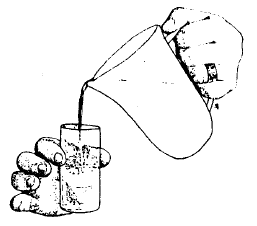
\includegraphics[width=\linewidth]{images/haptic}
		%\caption{\cite{johansson1987}}
	\end{figure}

\begin{itemize}
\item \textcolor{blue}{Kinesthésie}
\begin{itemize}
\setlength\itemsep{-0.2em}
\item \textcolor{blue}{Position}
\item \textcolor{blue}{Mouvement}
\item \textcolor{blue}{Force}
\item \textcolor{blue}{Résistance}
\end{itemize}
\end{itemize}

\end{multicols}	
	
\end{frame}
}

{
\setbeamertemplate{frame footer}{\cite{klatzky1990}}
\begin{frame}{Exploration haptique}
\begin{figure}
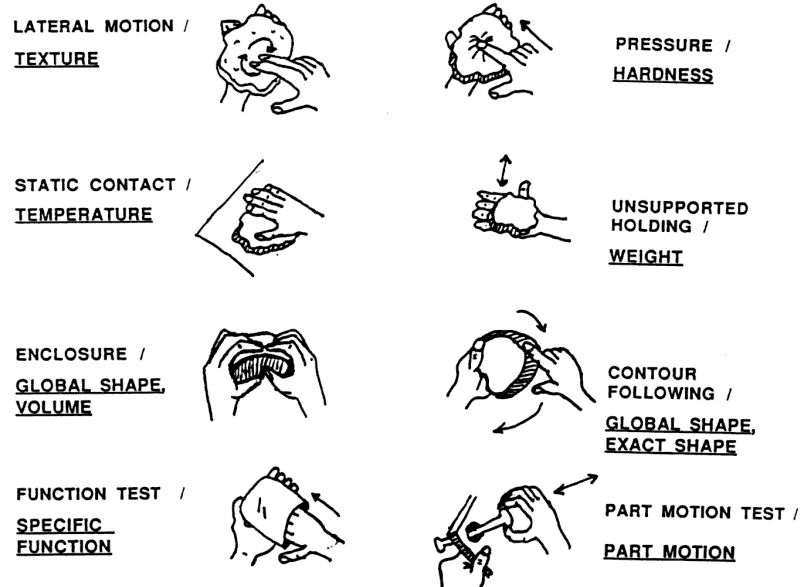
\includegraphics[width=9.5cm]{images/hapticExploration}
\end{figure}
\end{frame}
}

\subsection{Applications}
\begin{frame}{Exemples d'applications}
\begin{multicols}{2}
\begin{figure}
	\centering			
	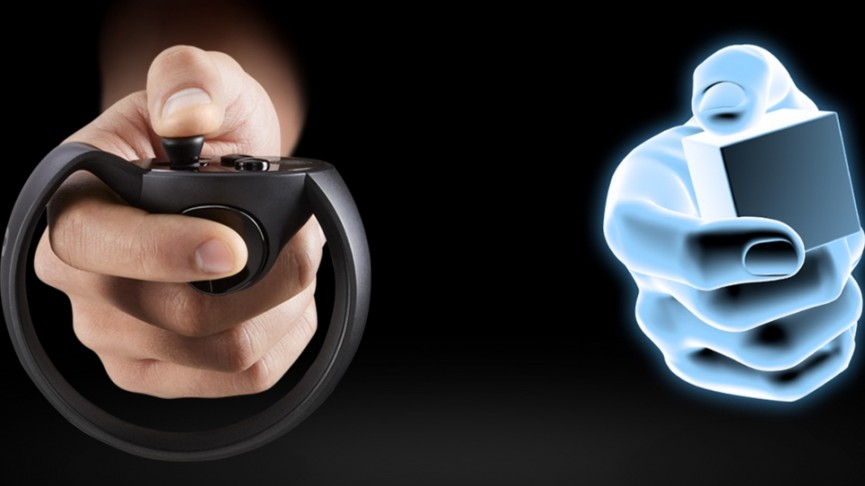
\includegraphics[width=4cm,height=2.7cm]{images/touch_vr}%{\copyright Nintendo}
	%\vspace{-0.5cm}
	\caption{Divertissement}
	\end{figure}
		\vspace{-0.7cm}	
	\begin{figure}	
	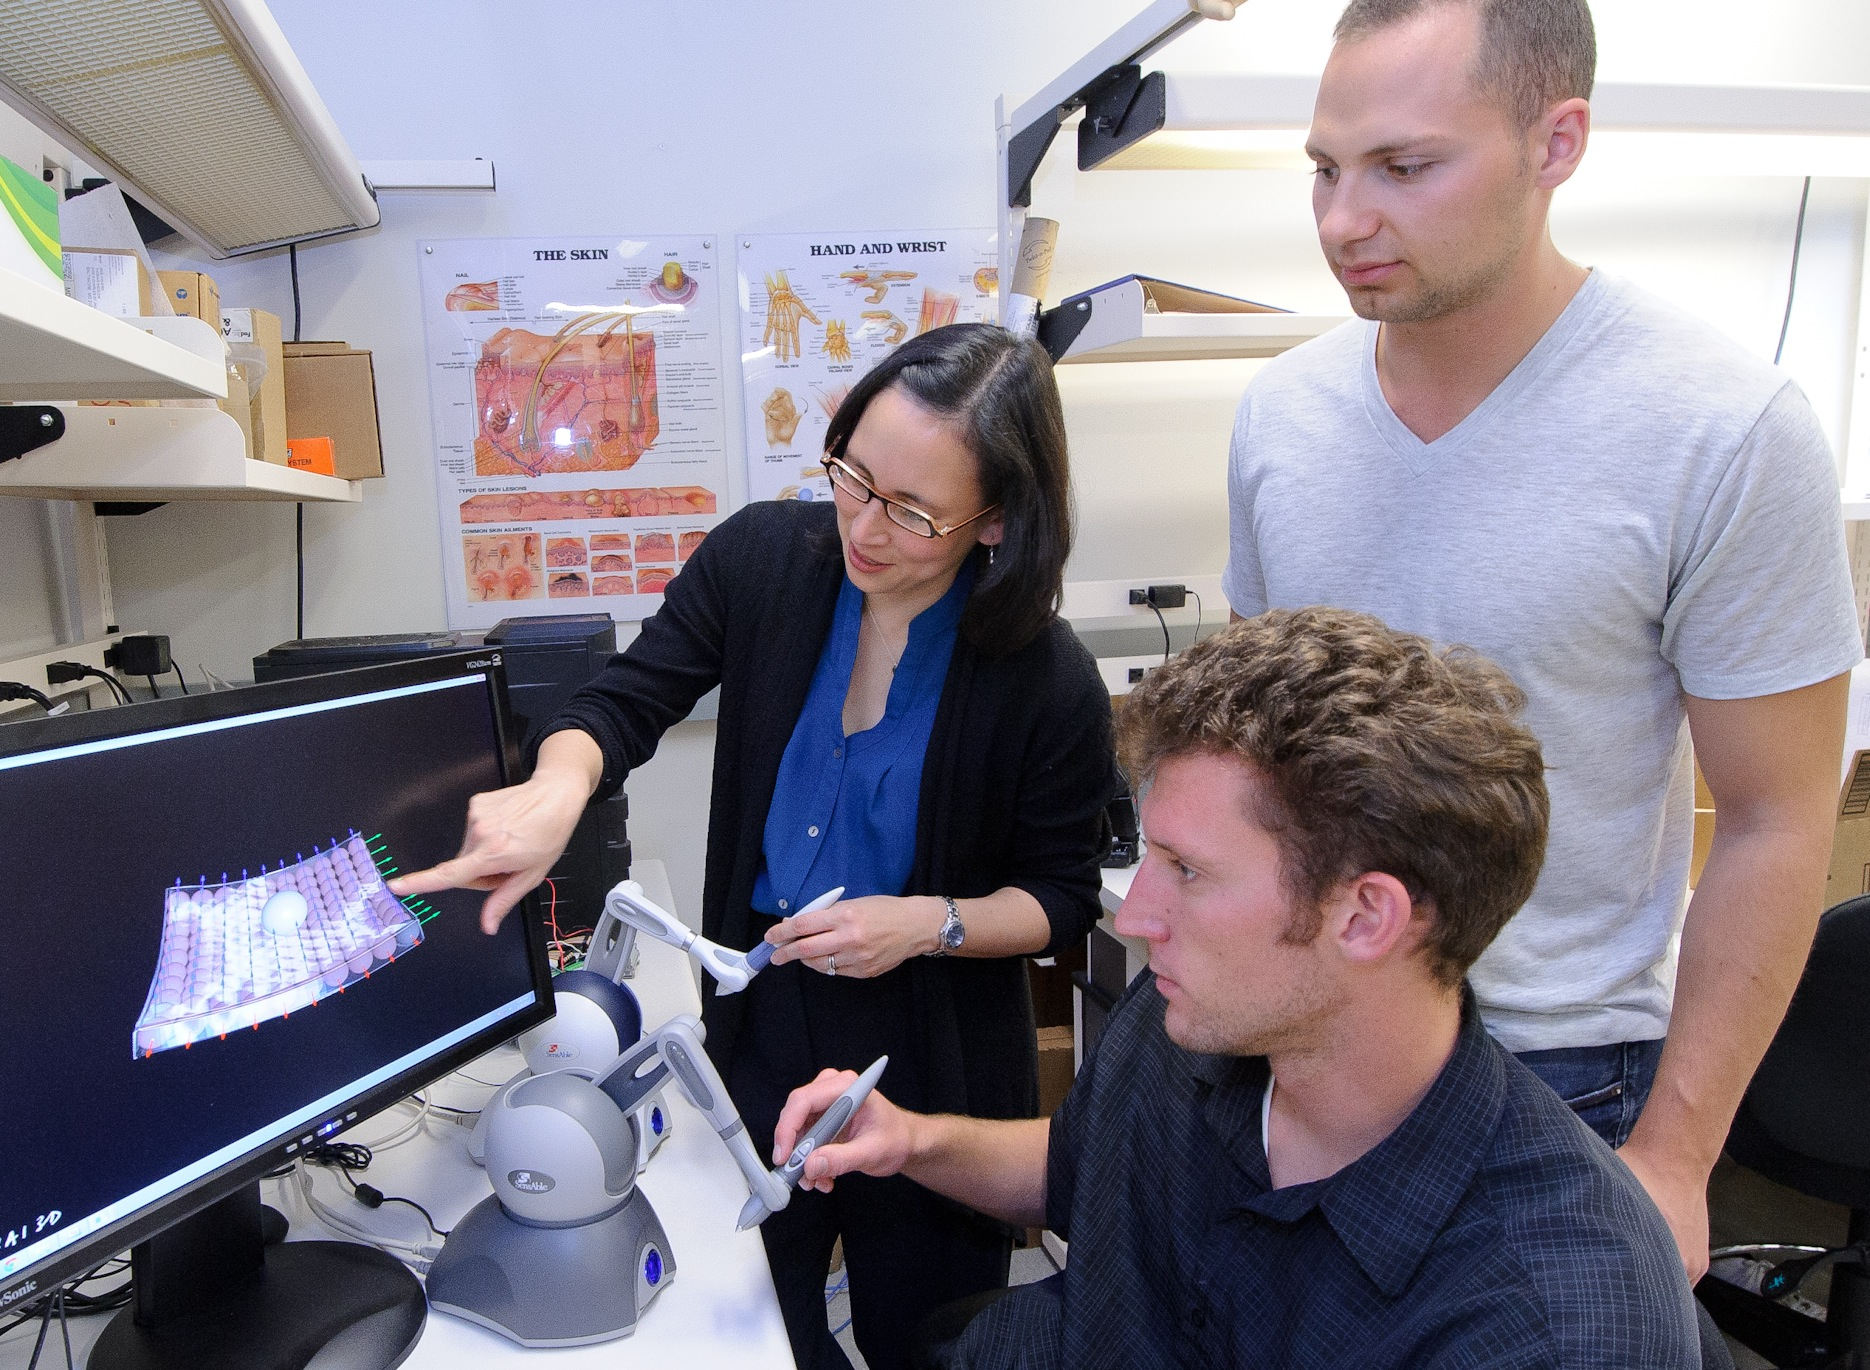
\includegraphics[width=4cm, height=2.7cm]{images/education}%{\copyright Stanford Charm Lab}
	%	\vspace{-0.5cm}
	\caption{Education}
	\end{figure}

\begin{figure}
	\centering			
	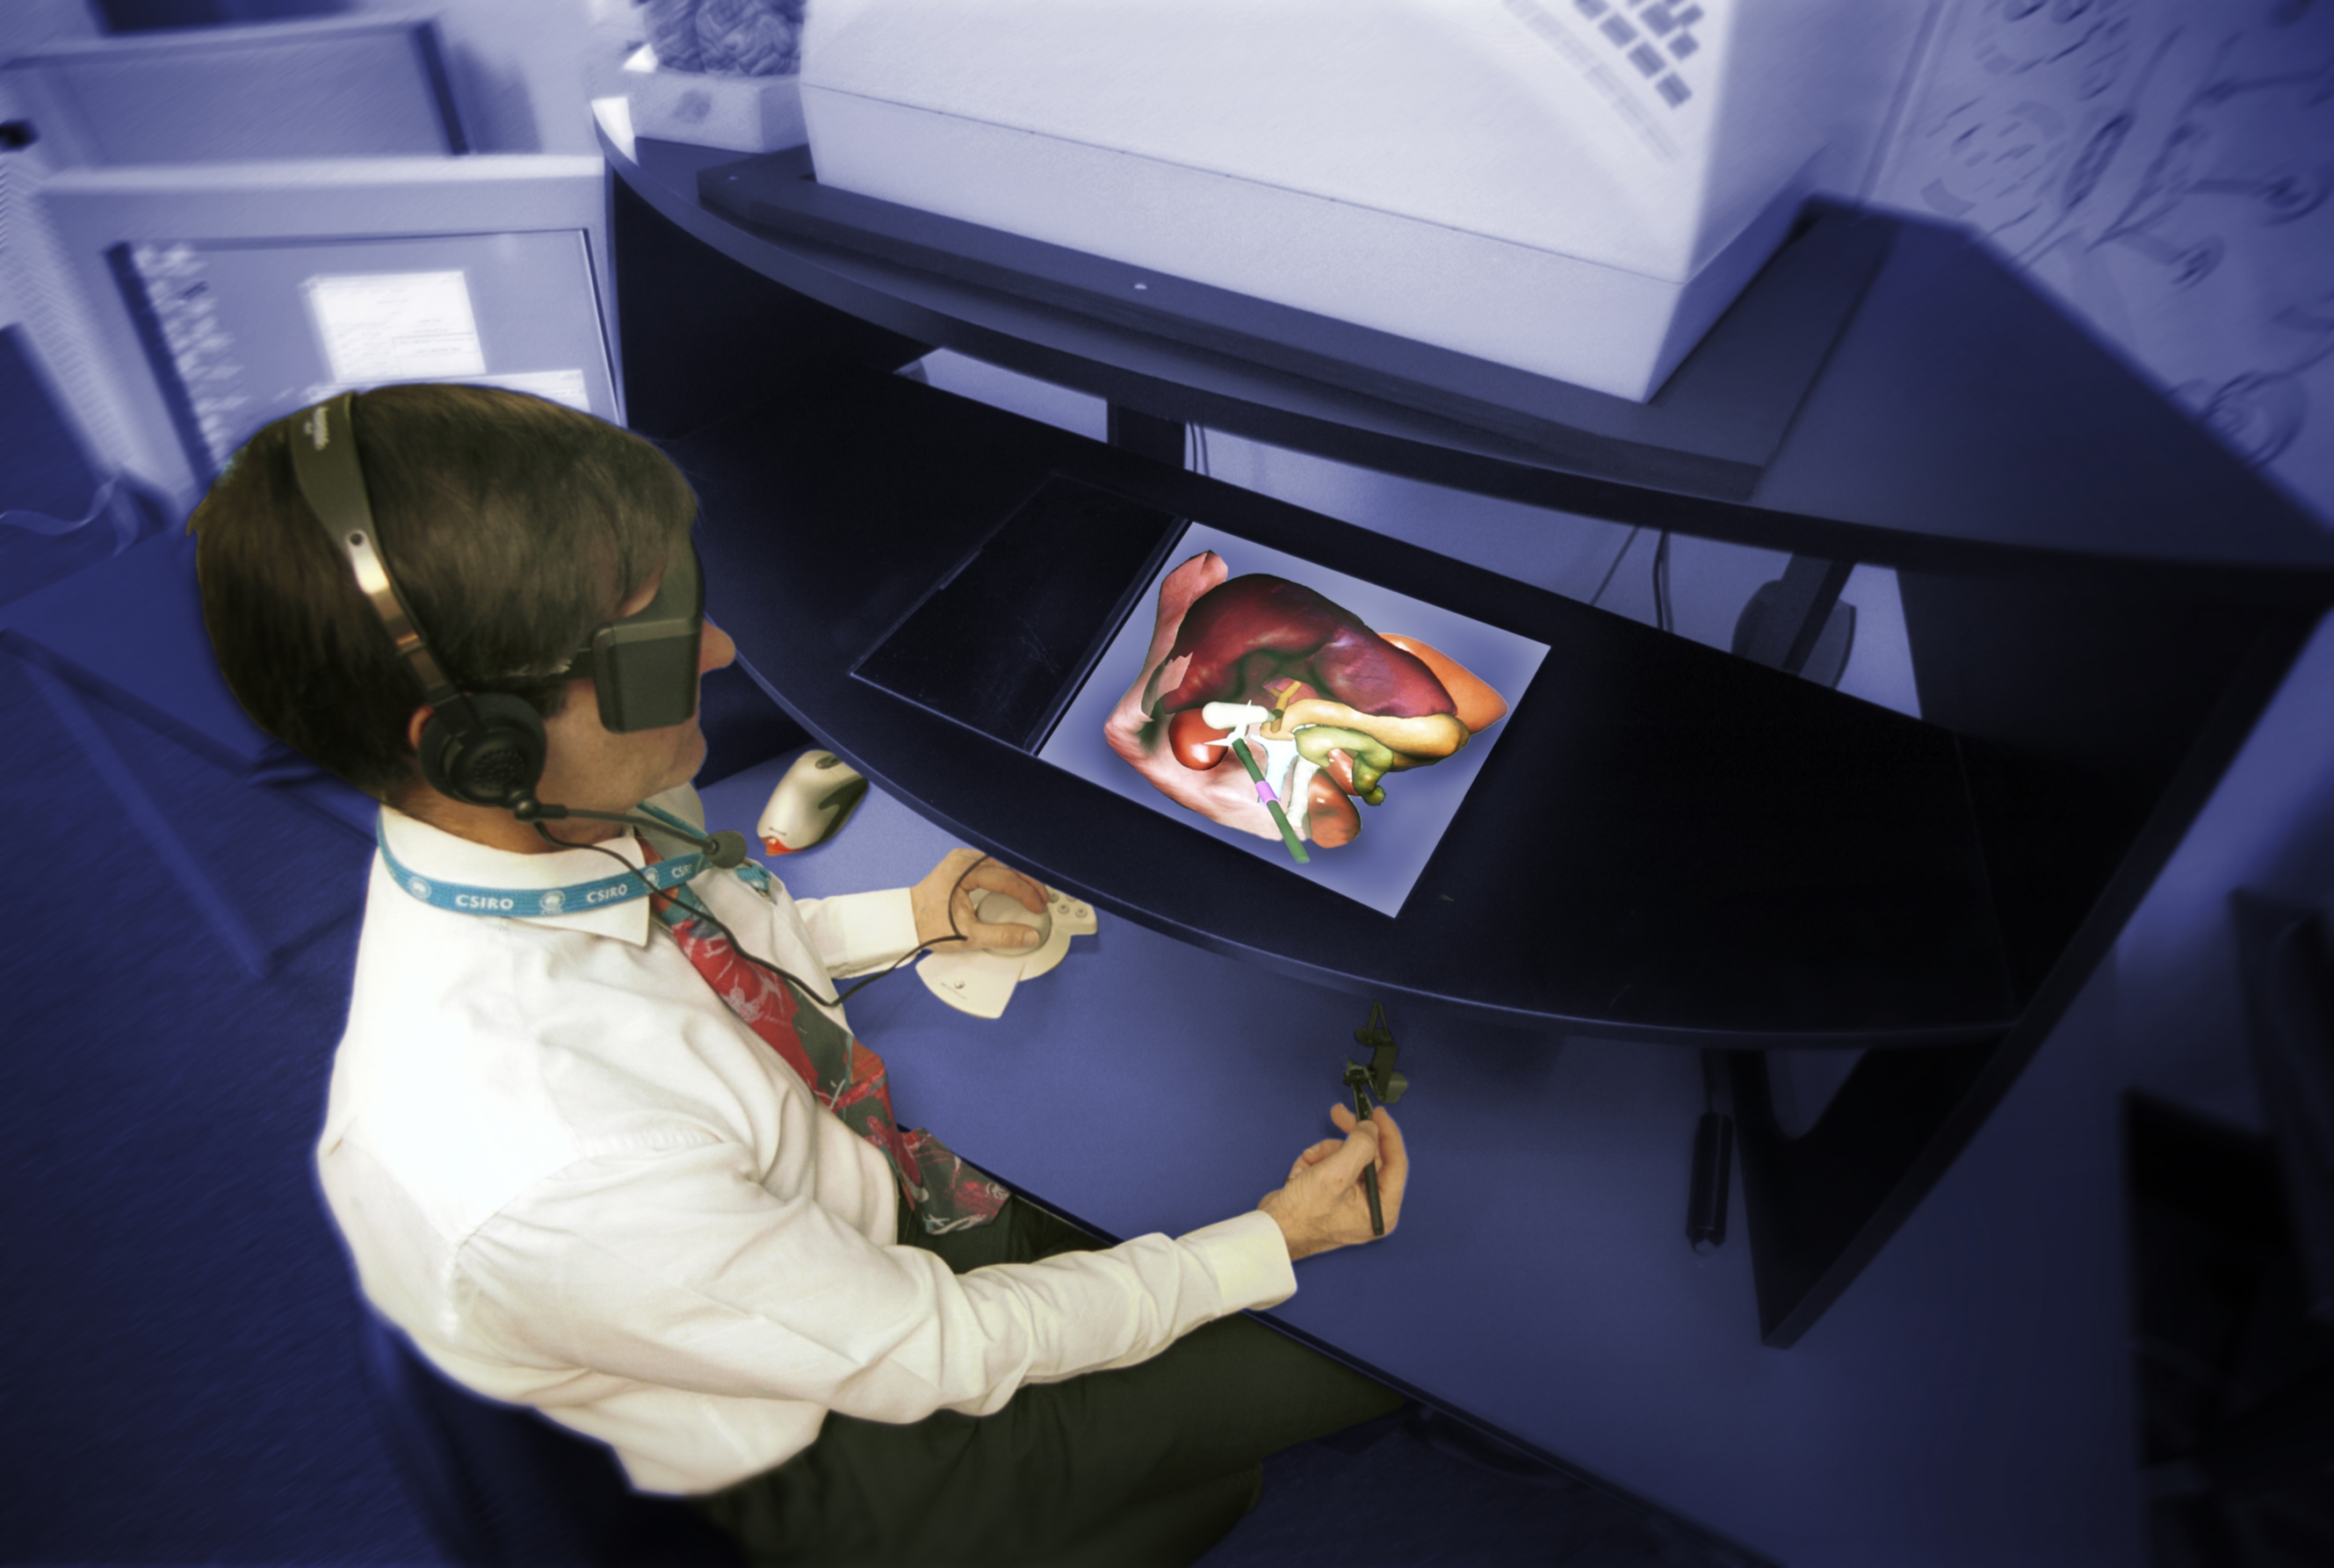
\includegraphics[width=4cm,height=2.7cm]{images/hapticSurgery}%{\copyright CSIRO}
	%	\vspace{-0.5cm}
	\caption{Médical}
		\end{figure}	
					\vspace{-1.5cm}	
	\begin{figure}
	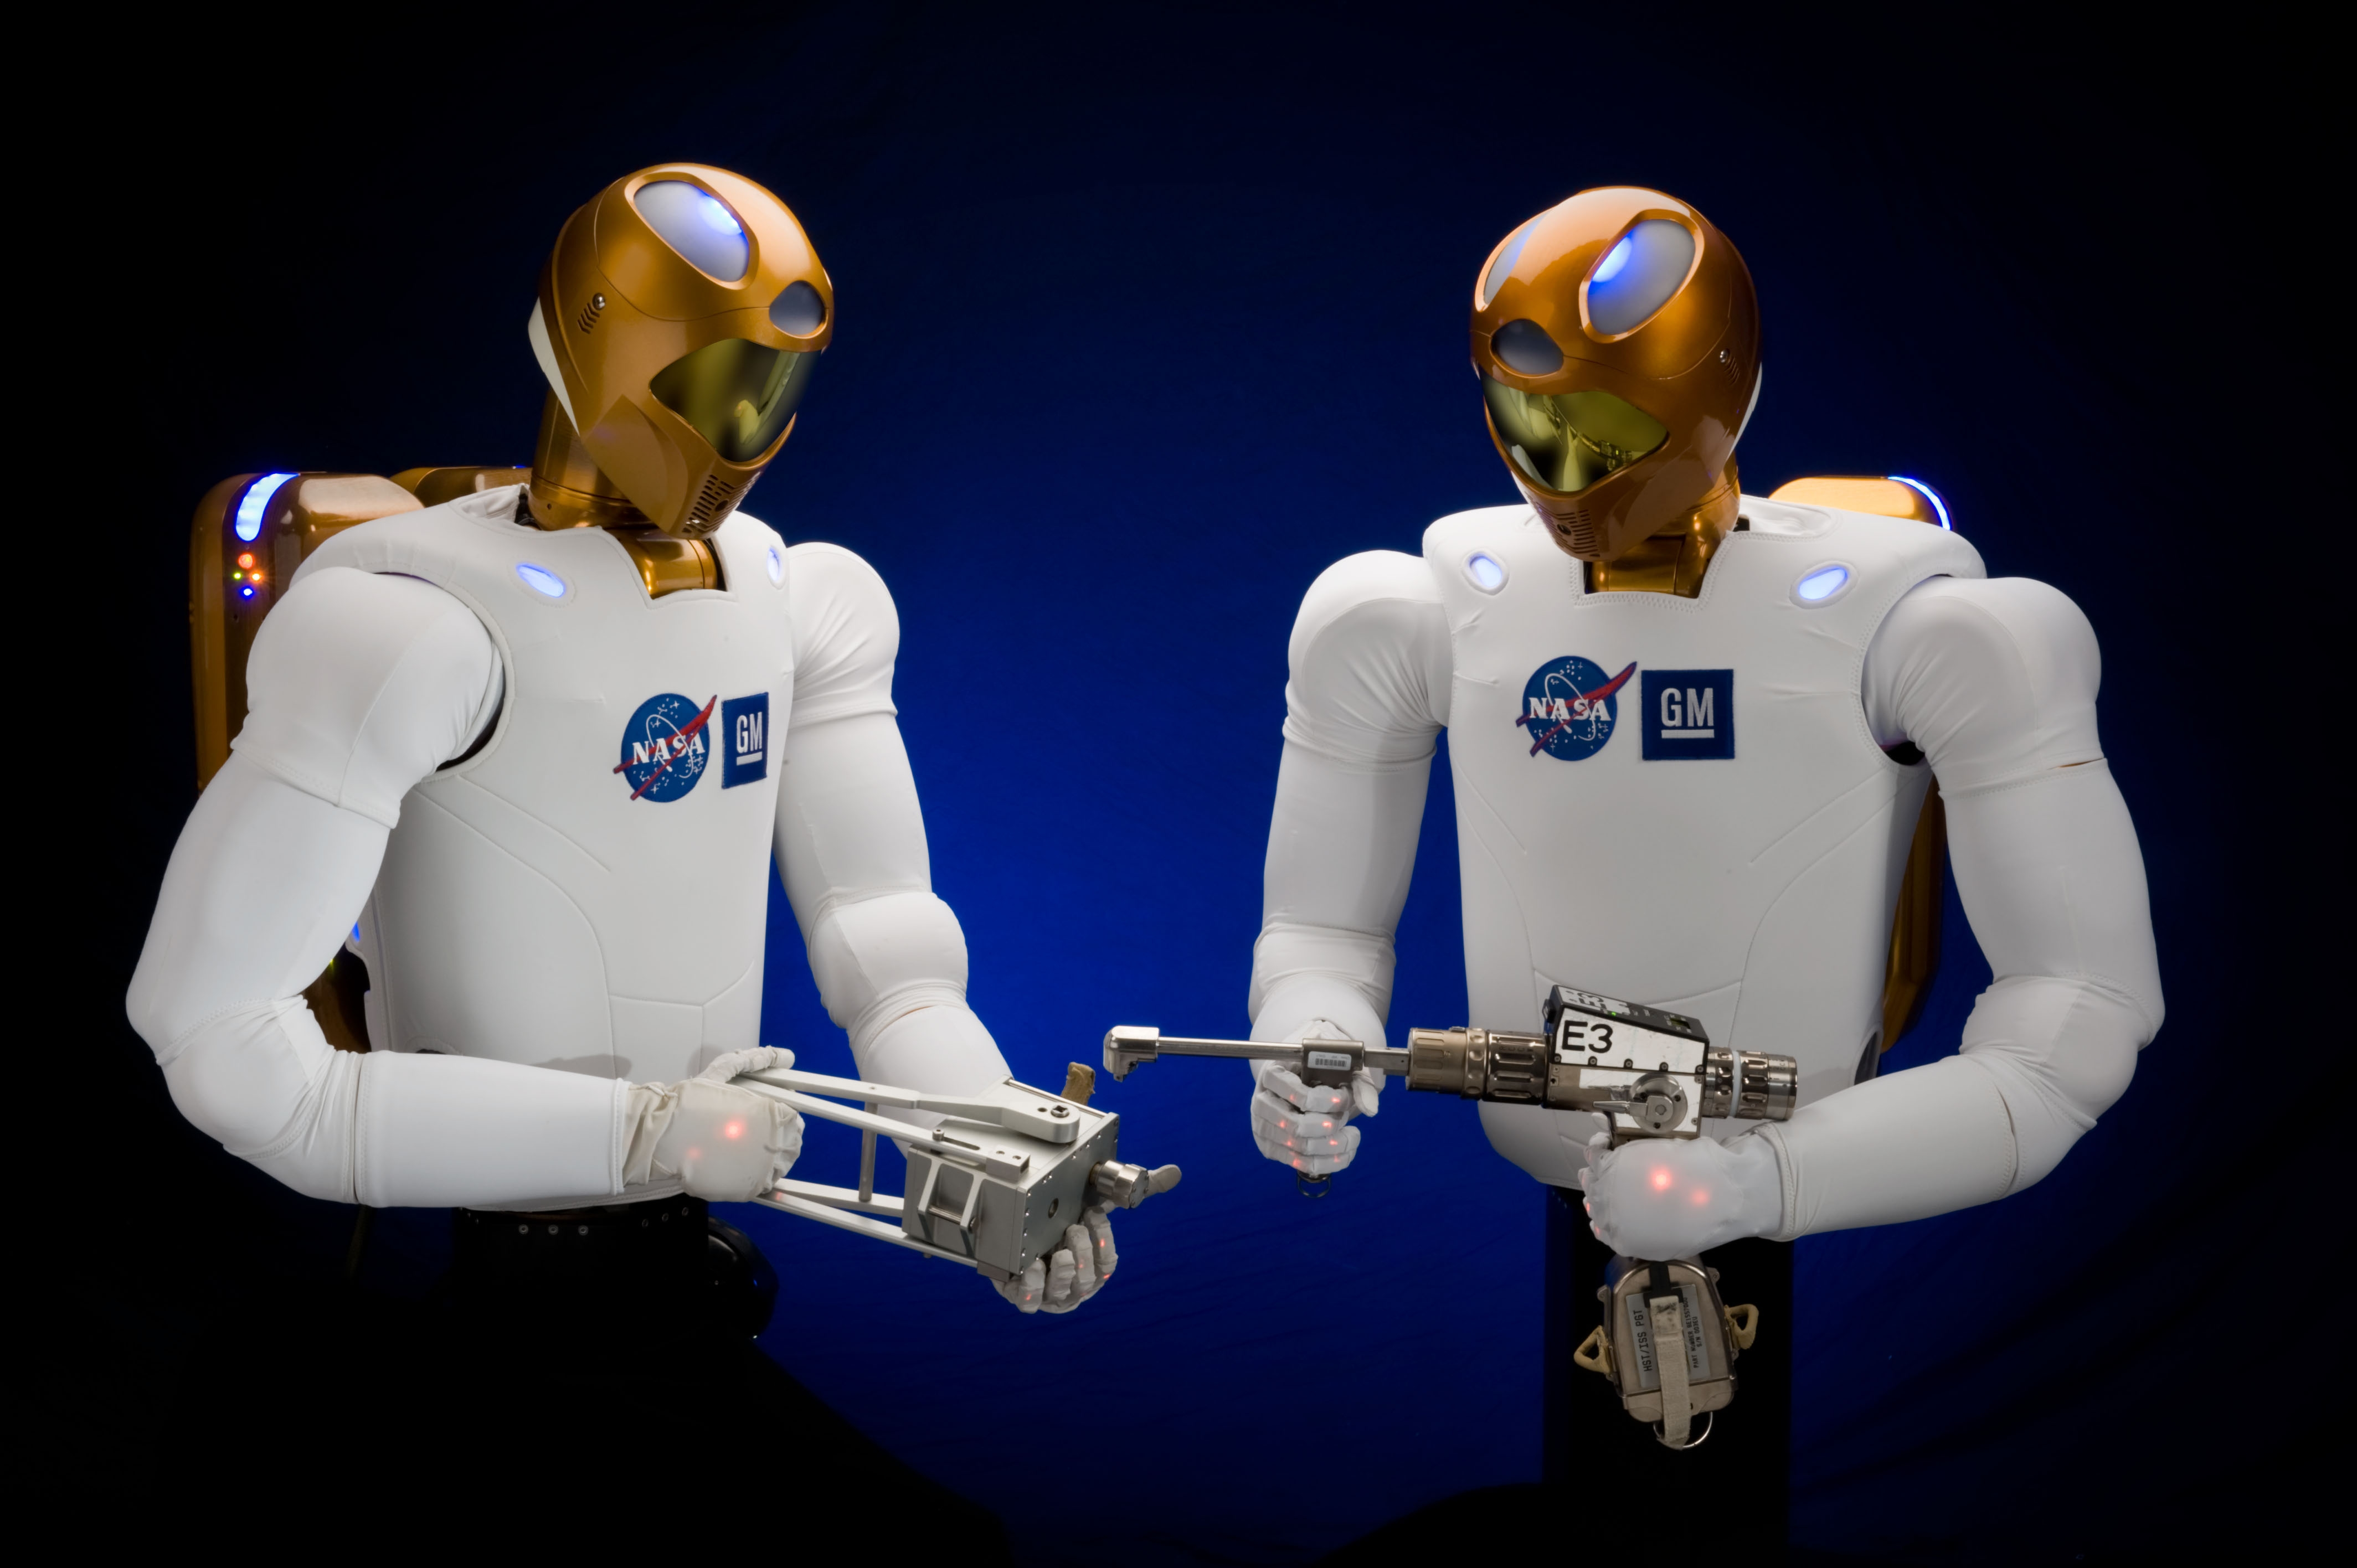
\includegraphics[width=4cm,height=2.7cm]{images/teleoperation}%{\copyright Nasa}
	%	\vspace{-0.5cm}
	\caption{Téléoperation}
	\end{figure}
	
\end{multicols}
\end{frame}

\begin{frame}{Flux de travail}

\begin{figure}
\centering
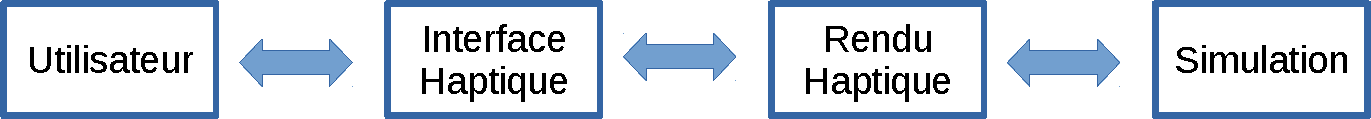
\includegraphics[width=\linewidth]{images/schema_haptique}	
\caption{Flux de travail pour l'interaction haptique}
		%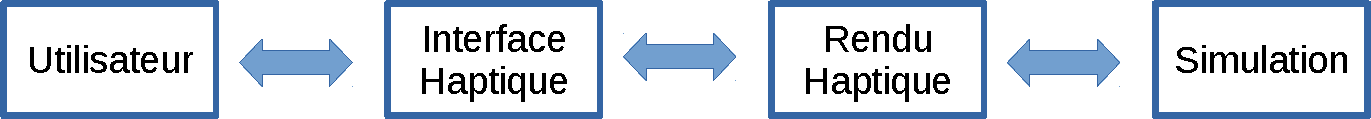
\includegraphics[width=4cm]{images/schema_haptique}{Johansson and Westling}
\end{figure}

\begin{itemize}
\item Utilisateur: contrôle l'interface haptique et ressent le retour haptique
\item Interface haptique: sert d'intermédiaire entre le monde réel et la simulation
\item Algorithme de rendu haptique: calcul le retour haptique à rendre via l'interface haptique
\item Simulation: représentation du monde virtuel ou distant
\end{itemize}	
\end{frame}